\documentclass[11pt]{article}
\usepackage[margin=1in]{geometry}
\usepackage{graphicx}
\usepackage{amsmath, amssymb}
\usepackage{booktabs}
\usepackage{hyperref}
\usepackage{caption}
\usepackage{xcolor}
\usepackage{float}
\hypersetup{colorlinks=true, linkcolor=blue, urlcolor=blue}
\graphicspath{{figs/}}

\title{Magic-Angle (Quasi-Transverse) Single-Mode Launch from \\
       Two HF Transmitter Sites:\\
       \large Geometry, Skip Geography, and Mode-Excitation Ratio}
\author{Christopher Stubbs}
\date{\today}

\begin{document}
\maketitle

\begin{abstract}
A vertical-linear emitter at any HF transmitter site has a
\emph{magic launch direction} along the local magnetic meridian for
which the launched wave is in QT (quasi-transverse) geometry --
$\hat{k} \perp \hat{B}$ at the bottomside ionosphere -- and the
launched E-vector aligns with the projection of the geomagnetic field
into the wave's perpendicular plane.  In that geometry, a vertical
antenna excites essentially only one of the two magneto-ionic
eigenmodes (O or X), and the suppression of the other can exceed
30~dB.  Adjacent (azimuth, elevation) pairs along the QT locus give
weaker but still useful mode discrimination.

This report documents the QT locus from two transmitter sites --
WWV-style co-located at Fort Collins, CO (mid-latitude, dip $\approx
66\textdegree$) and a hypothetical second site in Taipei, Taiwan (mid-
to-low latitude, dip $\approx 36\textdegree$) -- and where on the
ground rays launched along that locus arrive, separately for local
noon and local midnight.  Mode-excitation-ratio plots and the
resulting on-ground skip arcs are included.

The geometric ``magic point'' on the magnetic meridian (azimuth =
declination, elevation = $90\textdegree-\text{dip}$) is the only
direction with diverging mode-excitation ratio for an unmodified
vertical antenna.  Off the meridian, on the rest of the QT locus, the
ratio plateaus at $\approx +7\,$dB at FC and $\approx +1.5\,$dB at
Taipei -- modest but useful.
\end{abstract}


\section{Definitions and method}

\subsection*{QT locus}

For a vertical-linear emitter, the launched wave-normal $\hat{k}$ at
azimuth $A$ and elevation $\varepsilon$ is exactly perpendicular to
the local geomagnetic field $\hat{B}$ when
\begin{equation}
  \cos(A - \mathrm{decl}) = \tan\varepsilon \cdot \tan(\mathrm{dip})
  \label{eq:qt}
\end{equation}
where $\mathrm{dip}$ is the magnetic inclination (positive downward
in the northern hemisphere) and $\mathrm{decl}$ is the magnetic
declination (positive east of true north).  The locus has real
solutions only for $\varepsilon \le 90\textdegree - \mathrm{dip}$
(the \emph{cutoff elevation}); above that elevation, $\hat{k}$ is
inevitably tilted out of the perp-plane of $\hat{B}$ and pure-QT
geometry cannot be reached.

The locus consists of two branches symmetric about the magnetic
meridian.  As $\varepsilon$ rises from $0$ toward the cutoff, the
two branches sweep from near east/west (low elevation) toward the
magnetic meridian, where they merge.

\subsection*{Mode-excitation ratio}

In the QT-effective regime ($\theta_{kB}$ near $90\textdegree$,
$\beta\to 0$), the two magneto-ionic eigenmodes are nearly linear,
their major axes orthogonal in the perp-plane and aligned/anti-aligned
with the projection of $\hat{B}$ into the perp-plane.  A vertical-E
launch lands at angle $\alpha$ to that projection, and the energy
splits as
\begin{equation}
  f_O = \frac{\cos^2\alpha + \beta^2 \sin^2\alpha}{1+\beta^2}, \qquad
  f_X = \frac{\sin^2\alpha + \beta^2 \cos^2\alpha}{1+\beta^2}.
  \label{eq:fofx}
\end{equation}
For a vertical antenna along the QT locus, geometric algebra gives
\begin{equation}
  \alpha = \arccos\!\left(\cos(\mathrm{dip}) \sqrt{1 - \tan^2\varepsilon \tan^2(\mathrm{dip})}\right),
\end{equation}
which equals the local dip at low elevation (the off-meridian
plateau) and falls to zero at the cutoff (perfect alignment with the
O-mode axis on the magnetic meridian).  The $f_X/f_O$ dB ratio is
$10\log_{10}(\tan^2\alpha)$ in the deep-QT limit.

\subsection*{Ray tracing}

Skip-distance and landing-point calculations use PHaRLAP's
\texttt{raytrace\_3d} on a 3-D WGS84 spherical-Earth IRI-2020
ionosphere with an IGRF-2020 magnetic-field model.  Up to three hops
are traced; for each (frequency, branch, elevation) launch on the QT
locus, the brightest-by-total-dB arriving ray is recorded along with
its mode-class label, ground touchdown point, receiver-side $b/a$,
and number of ground bounces.

Time of day enters through the ionosphere: local noon and local
midnight at the path midpoint produce different IRI conditions, so
the same launch geometry produces different landing arcs.


\section{Mode-excitation-ratio geometry}

\begin{figure}[H]
\centering
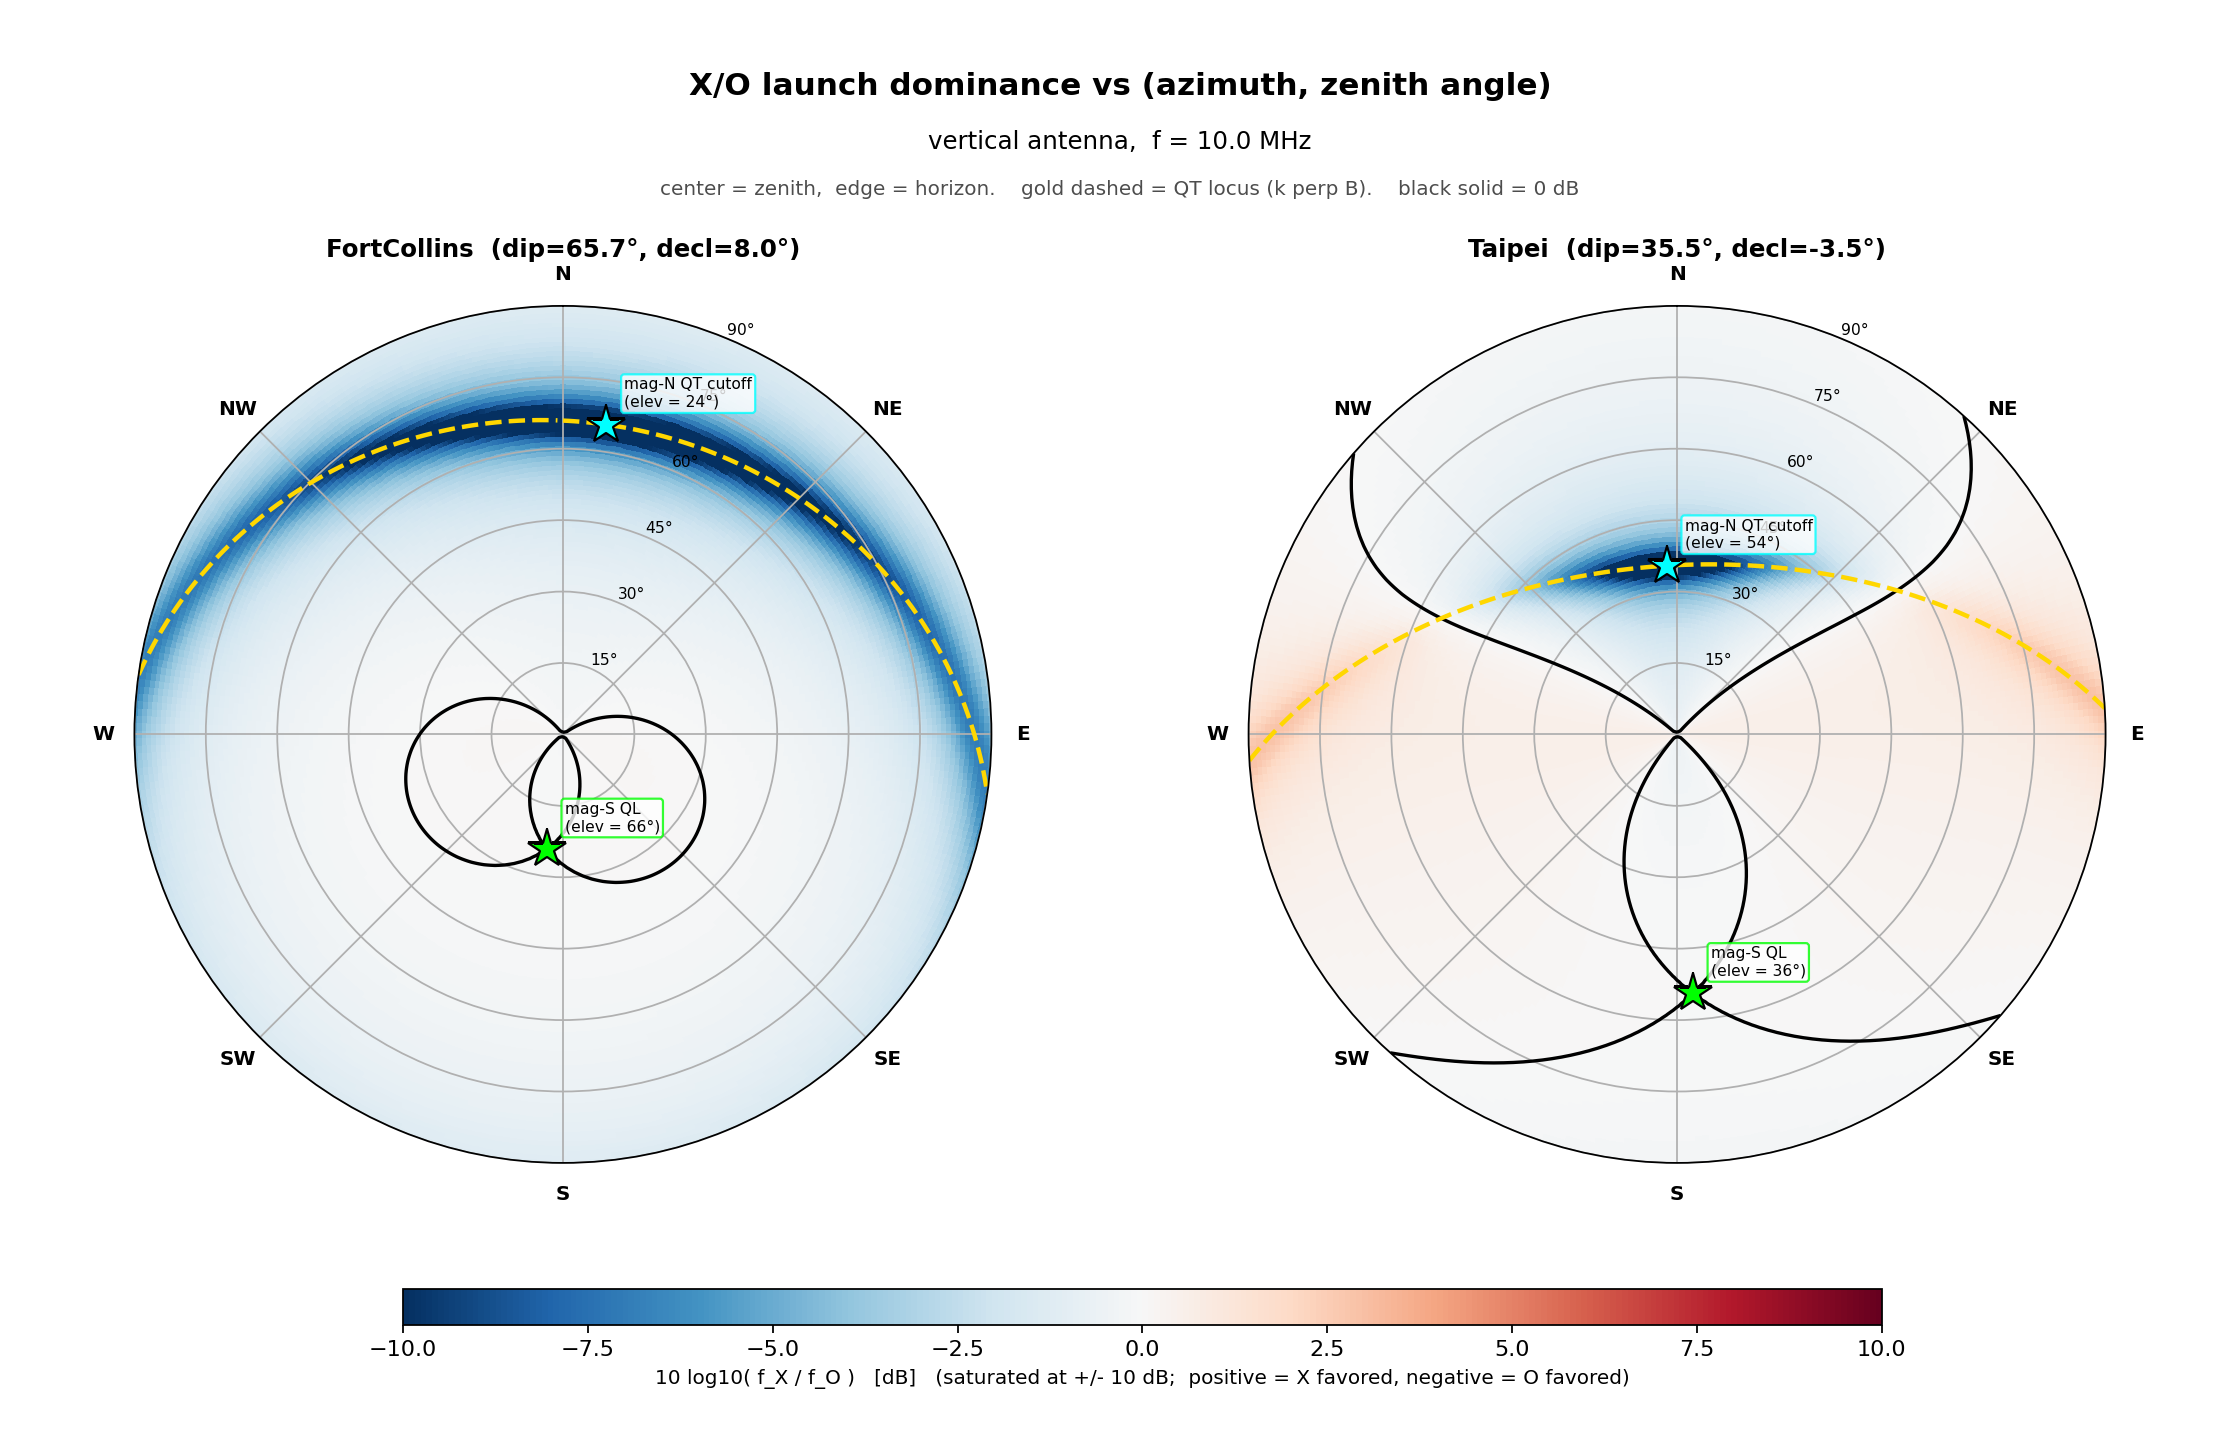
\includegraphics[width=0.95\textwidth]{qt_polar_map_FC_Taipei.png}
\caption{Polar map of the X/O launch-coupling ratio $10\log_{10}(f_X/f_O)$
for a vertical-linear emitter, at $f=10$\,MHz.  Each panel uses the
``looking down at the sky'' convention: azimuth runs clockwise from
true north (top), and the radial coordinate is zenith angle (centre =
straight up, edge = horizon).  Color encodes the dB ratio (red:
X-favored, blue: O-favored, white: 50/50).  \textbf{Gold dashed} = QT
locus where $\hat{k}\!\perp\!\hat{B}$.  \textbf{Cyan star} =
magnetic-N QT cutoff (the magic point, $\alpha\to 0$, deep blue).
\textbf{Lime star} = magnetic-S QL antiparallel point (modes are
purely circular here; vertical antenna gives 50/50 regardless).
At Fort Collins (left, dip $\approx 66\textdegree$) the QT locus is a
small arc near the horizon converging on mag-N at zenith angle
$\approx 66\textdegree$; the deepest mode purity is concentrated very
close to that single direction.  At Taipei (right, dip $\approx
36\textdegree$) the locus spans much wider zenith angles and the
contrast is shallower.}
\label{fig:polar}
\end{figure}

\begin{figure}[H]
\centering
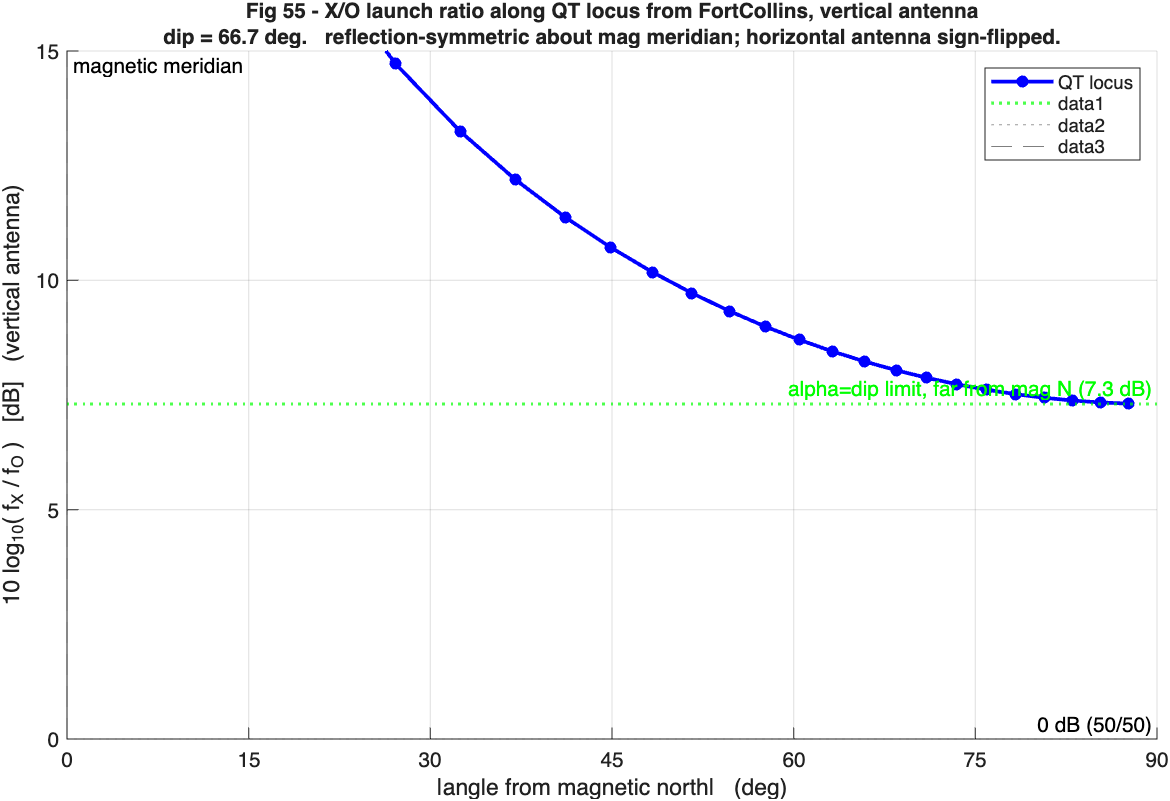
\includegraphics[width=0.85\textwidth]{qt_mode_ratio_vs_azimuth.png}
\caption{Signed mode-launch ratio $10\log_{10}(f_X/f_O)$ for a vertical
antenna, plotted vs.\ $|$angle from magnetic north$|$ along the QT
locus from Fort Collins.  East and west branches are reflection-
symmetric and folded onto a single curve.  Far from the magnetic
meridian (large angle off mag-N) the ratio plateaus at $+7$\,dB
($\alpha = \mathrm{dip} = 66\textdegree$); approaching the magnetic
meridian, the ratio dives toward $-\infty$ (pure O launch) where the
two QT branches merge at the cutoff elevation
$90\textdegree-\mathrm{dip} = 24\textdegree$.  Negative dB = O-mode
favored; positive dB = X-mode favored; horizontal antenna would be
sign-flipped.}
\label{fig:ratio_vs_az}
\end{figure}

\begin{figure}[H]
\centering
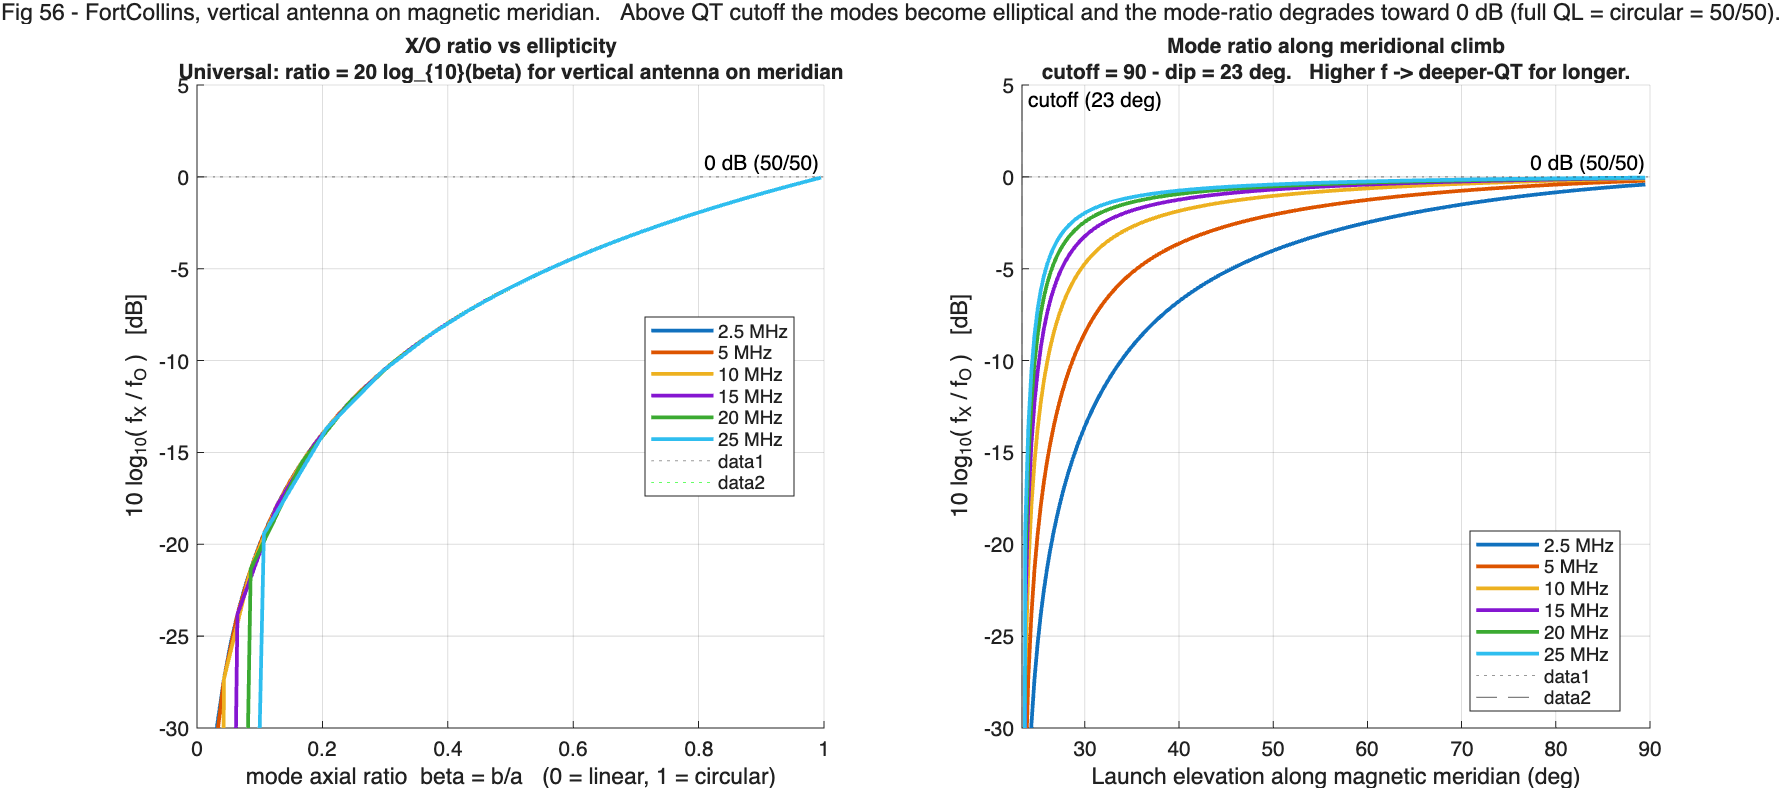
\includegraphics[width=0.95\textwidth]{qt_mode_ratio_vs_ellipticity.png}
\caption{Mode-ratio $10\log_{10}(f_X/f_O)$ versus the local
magneto-ionic axial ratio $\beta=b/a$ along the magnetic-meridian
launch from Fort Collins.  Each curve is one frequency $f \in \{2.5,
5, 10, 15, 20, 25\}$\,MHz.  \emph{Left:} ratio vs.\ $\beta$ collapses
onto a universal curve $20\log_{10}(\beta)$ regardless of frequency
-- only the geometry matters.  \emph{Right:} ratio vs.\ launch
elevation along the meridian -- different per frequency because Y
$=f_H/f$ enters the Appleton--Hartree axial ratio.  Higher
frequencies stay in deeper-QT (smaller $\beta$) longer as the
elevation rises, so the discrimination degrades more slowly at higher
HF.}
\label{fig:ratio_vs_beta}
\end{figure}


\section{Skip geography from Fort Collins}

Fort Collins, CO ($40.68\textdegree$N, $105.04\textdegree$W).
Magnetic dip $\approx 66\textdegree$, declination $\approx
+8\textdegree$.  QT cutoff elevation $\approx 24\textdegree$;
magnetic-meridian magic-point azimuth $\approx 8\textdegree$.

\begin{figure}[H]
\centering
\begin{minipage}{0.49\textwidth}\centering
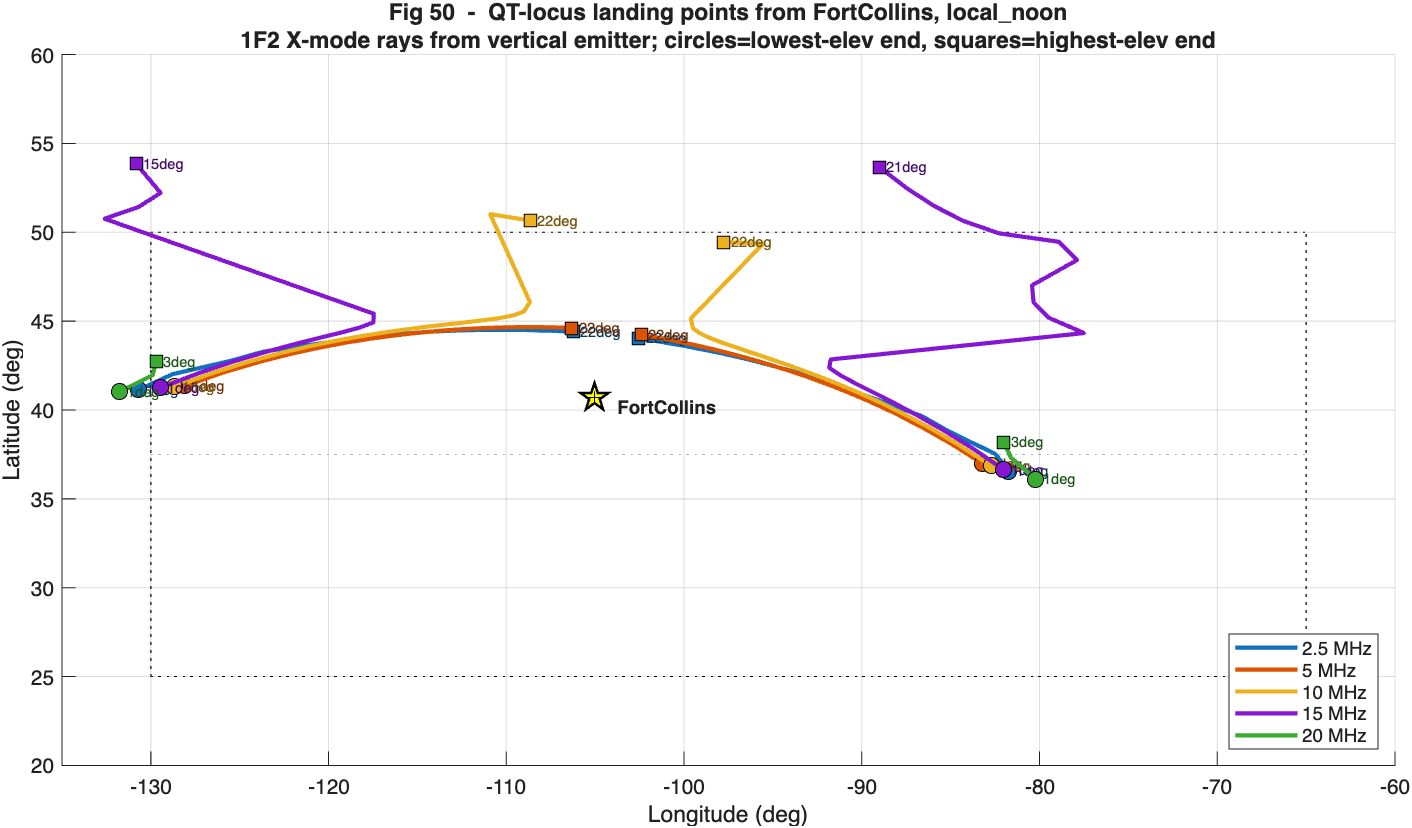
\includegraphics[width=\textwidth]{fc_qt_map_noon.png}\\
\textbf{(a)} local noon
\end{minipage}\hfill
\begin{minipage}{0.49\textwidth}\centering
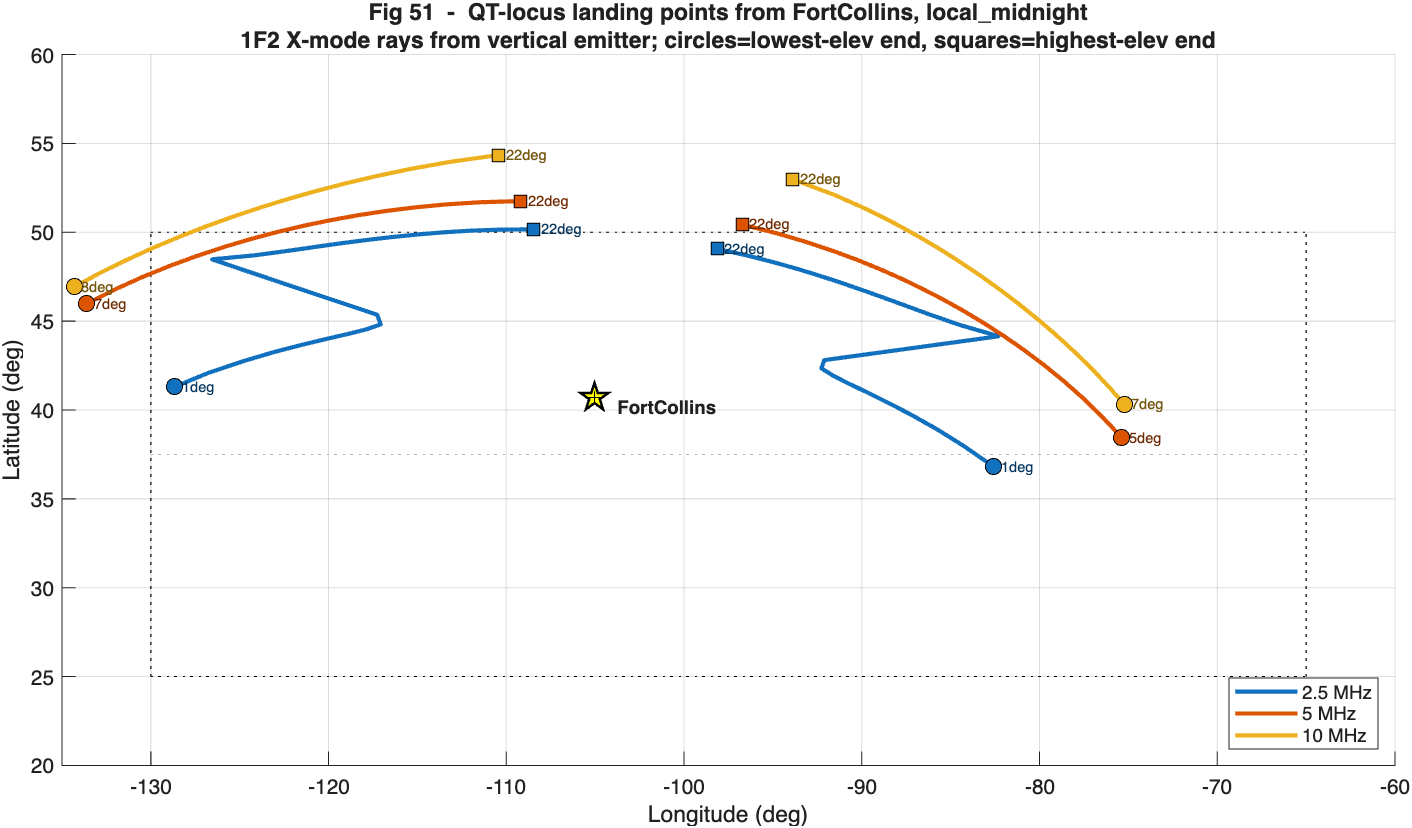
\includegraphics[width=\textwidth]{fc_qt_map_midnight.png}\\
\textbf{(b)} local midnight
\end{minipage}
\caption{QT-locus brightest-mode landings from Fort Collins for
$f \in \{2.5, 5, 10, 15, 20, 25\}$\,MHz.  Each colored arc traces
where rays land on the ground as the launch elevation walks the QT
locus from low (long range, far end of arc) to near-cutoff (short
range, the magnetic-meridian end).  Marker shapes encode hop count
(circle = 1-hop, square = 2-hop, triangle = 3-hop).  Mode-class
labels indicate which ionospheric layer each ray reflected from (E,
F1, F2).  Both east-of-meridian and west-of-meridian branches are
shown.  At noon, the D-region absorption kills the lower-MHz arcs
(the 2.5\,MHz curve is heavily suppressed); at midnight, all bands
arrive cleanly.}
\label{fig:fc_maps}
\end{figure}

\begin{figure}[H]
\centering
\begin{minipage}{0.49\textwidth}\centering
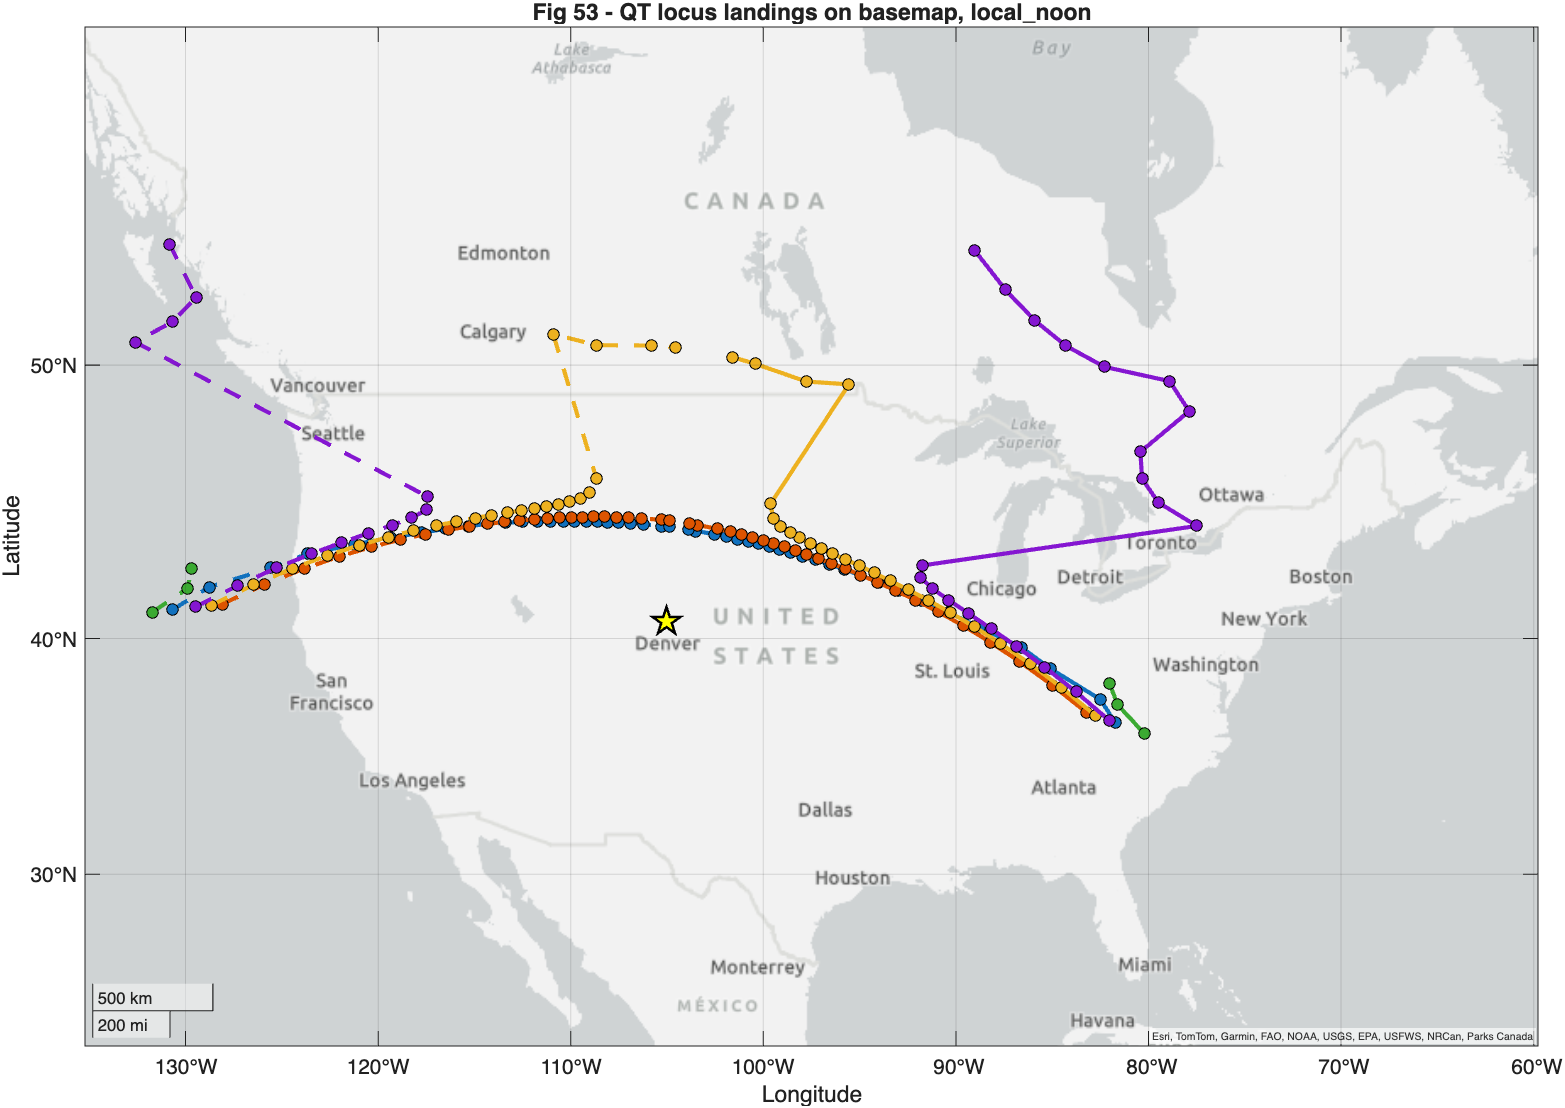
\includegraphics[width=\textwidth]{fc_qt_basemap_noon.png}\\
\textbf{(a)} local noon
\end{minipage}\hfill
\begin{minipage}{0.49\textwidth}\centering
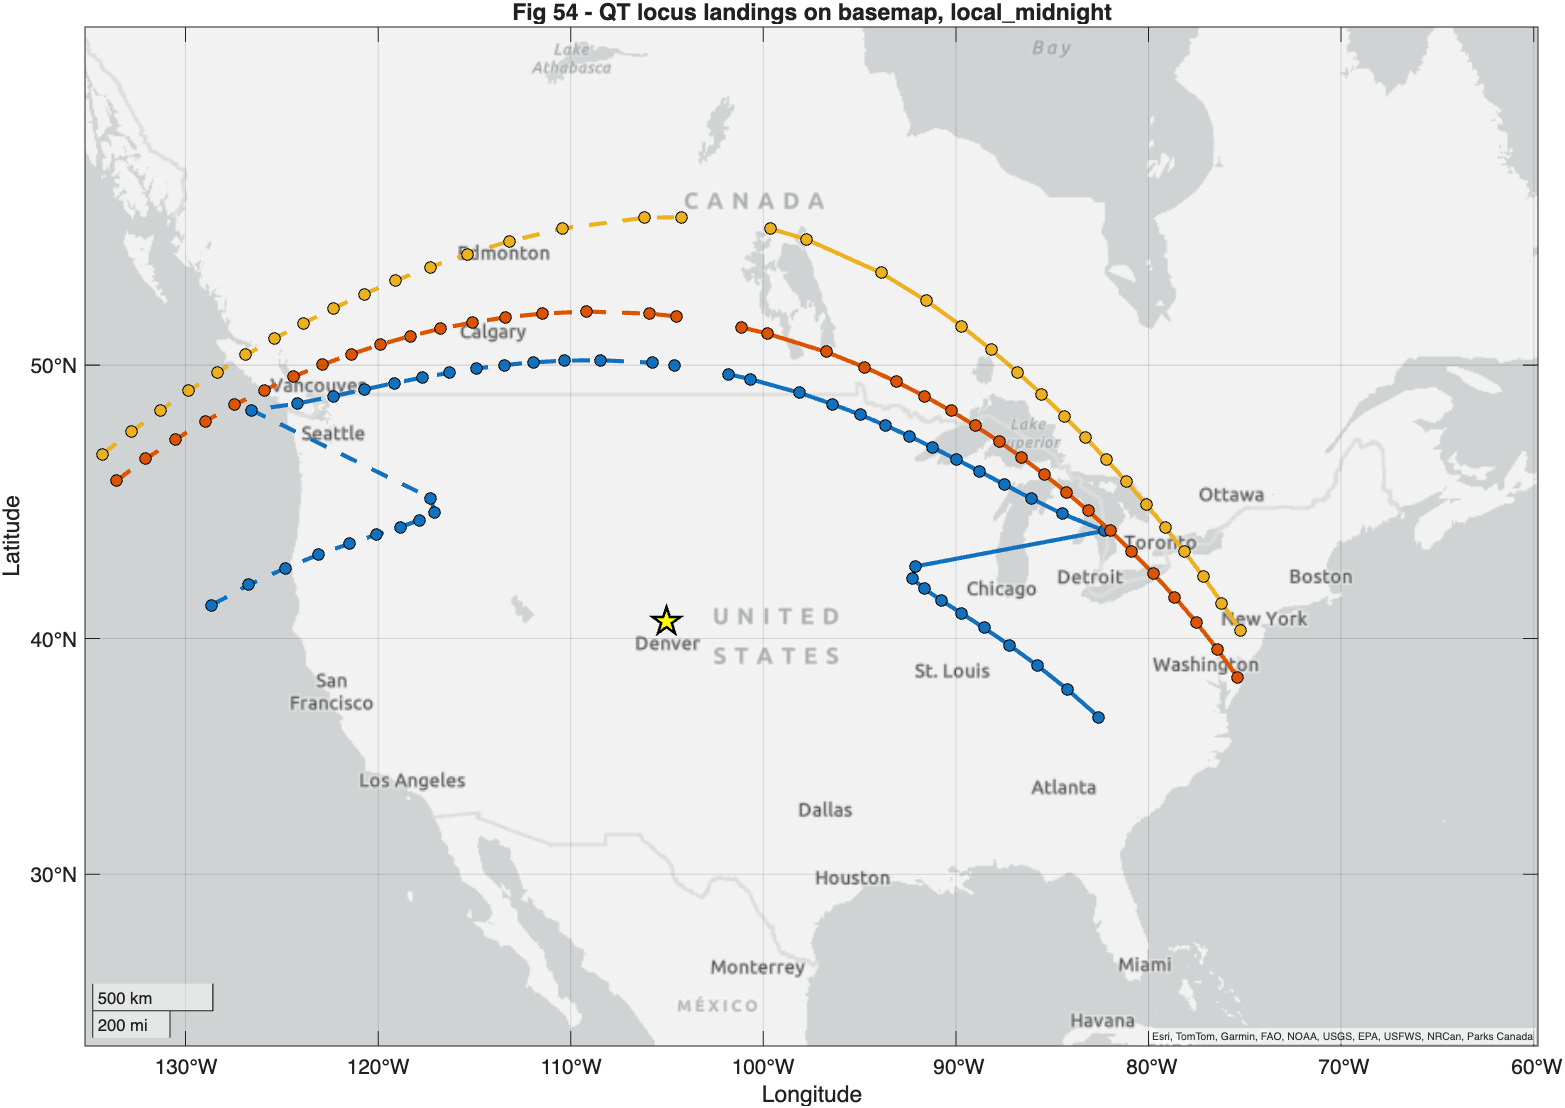
\includegraphics[width=\textwidth]{fc_qt_basemap_midnight.png}\\
\textbf{(b)} local midnight
\end{minipage}
\caption{Same data as
Figure~\ref{fig:fc_maps}, overlaid on a real terrain basemap via
MATLAB \texttt{geoaxes}.  Useful for identifying which actual
receiver sites (KiwiSDR locations, university observatories, amateur
clubs) sit on the magic locus.}
\label{fig:fc_basemaps}
\end{figure}

\begin{table}[H]
\centering
\caption{Brightest QT-locus ray per frequency, FC, local noon (east
branch).  $f_X/f_O$ ratio is the geometric mode-coupling ratio for a
vertical antenna; loss is the total path attenuation
$L_\mathrm{free}+L_\mathrm{abs}+L_\mathrm{ground}$.  Bands where
$L_\mathrm{abs}$ from D-region absorption swamps the budget (e.g.\
2.5\,MHz noon) come out very negative.}
\begin{tabular}{rrrlrrrrr}
\toprule
$f$ & $\varepsilon$ & az & class & range & $b/a$ & $f_X/f_O$ & loss & lat,lon \\
MHz & deg & deg & & approx & & dB & dB & deg \\
\midrule
2.5 & 23.2 & 13.1 & 1E & 1-hop & 0.82 & +28.2 & -288.8 & 44.2, -103.9 \\
5.0 & 23.2 & 13.1 & 1E & 1-hop & 0.91 & +28.2 & -156.2 & 44.4, -103.8 \\
10.0 & 15.0 & 59.1 & 1E & 1-hop & 0.88 & +9.7 & -136.0 & 43.7, -97.6 \\
15.0 & 8.0 & 78.5 & 1E & 1-hop & 0.82 & +7.9 & -134.5 & 42.0, -91.2 \\
20.0 & 2.0 & 92.8 & 1E & 1-hop & 0.35 & +7.3 & -137.8 & 37.3, -81.6 \\
\bottomrule
\end{tabular}

\label{tab:fc_noon}
\end{table}

\begin{table}[H]
\centering
\caption{Same as Table~\ref{tab:fc_noon} but at local midnight.}
\begin{tabular}{rrrlrrrrr}
\toprule
$f$ & $\varepsilon$ & az & class & range & $b/a$ & $f_X/f_O$ & loss & lat,lon \\
MHz & deg & deg & & approx & & dB & dB & deg \\
\midrule
2.5 & 23.2 & 13.1 & 1F2 & 1-hop & 0.79 & +28.2 & -135.9 & 49.7, -101.8 \\
5.0 & 23.2 & 13.1 & 1F2 & 1-hop & 0.89 & +28.2 & -124.1 & 51.2, -101.1 \\
10.0 & 23.2 & 13.1 & 1F2 & 1-hop & 0.93 & +28.2 & -125.5 & 54.3, -99.6 \\
\bottomrule
\end{tabular}

\label{tab:fc_midnight}
\end{table}


\section{Skip geography from Taipei}

Taipei, Taiwan ($25.03\textdegree$N, $121.57\textdegree$E).  Magnetic
dip $\approx 36\textdegree$, declination $\approx -3.5\textdegree$
(west).  QT cutoff elevation $\approx 54\textdegree$ (much higher
than at FC), so the QT locus spans a much larger range of launch
elevations and azimuths.  But the off-meridian plateau ratio
$10\log_{10}(\tan^2 36\textdegree) \approx +1.5\,$dB is much
shallower -- mode discrimination away from the magnetic meridian is
weak.

\begin{figure}[H]
\centering
\begin{minipage}{0.49\textwidth}\centering
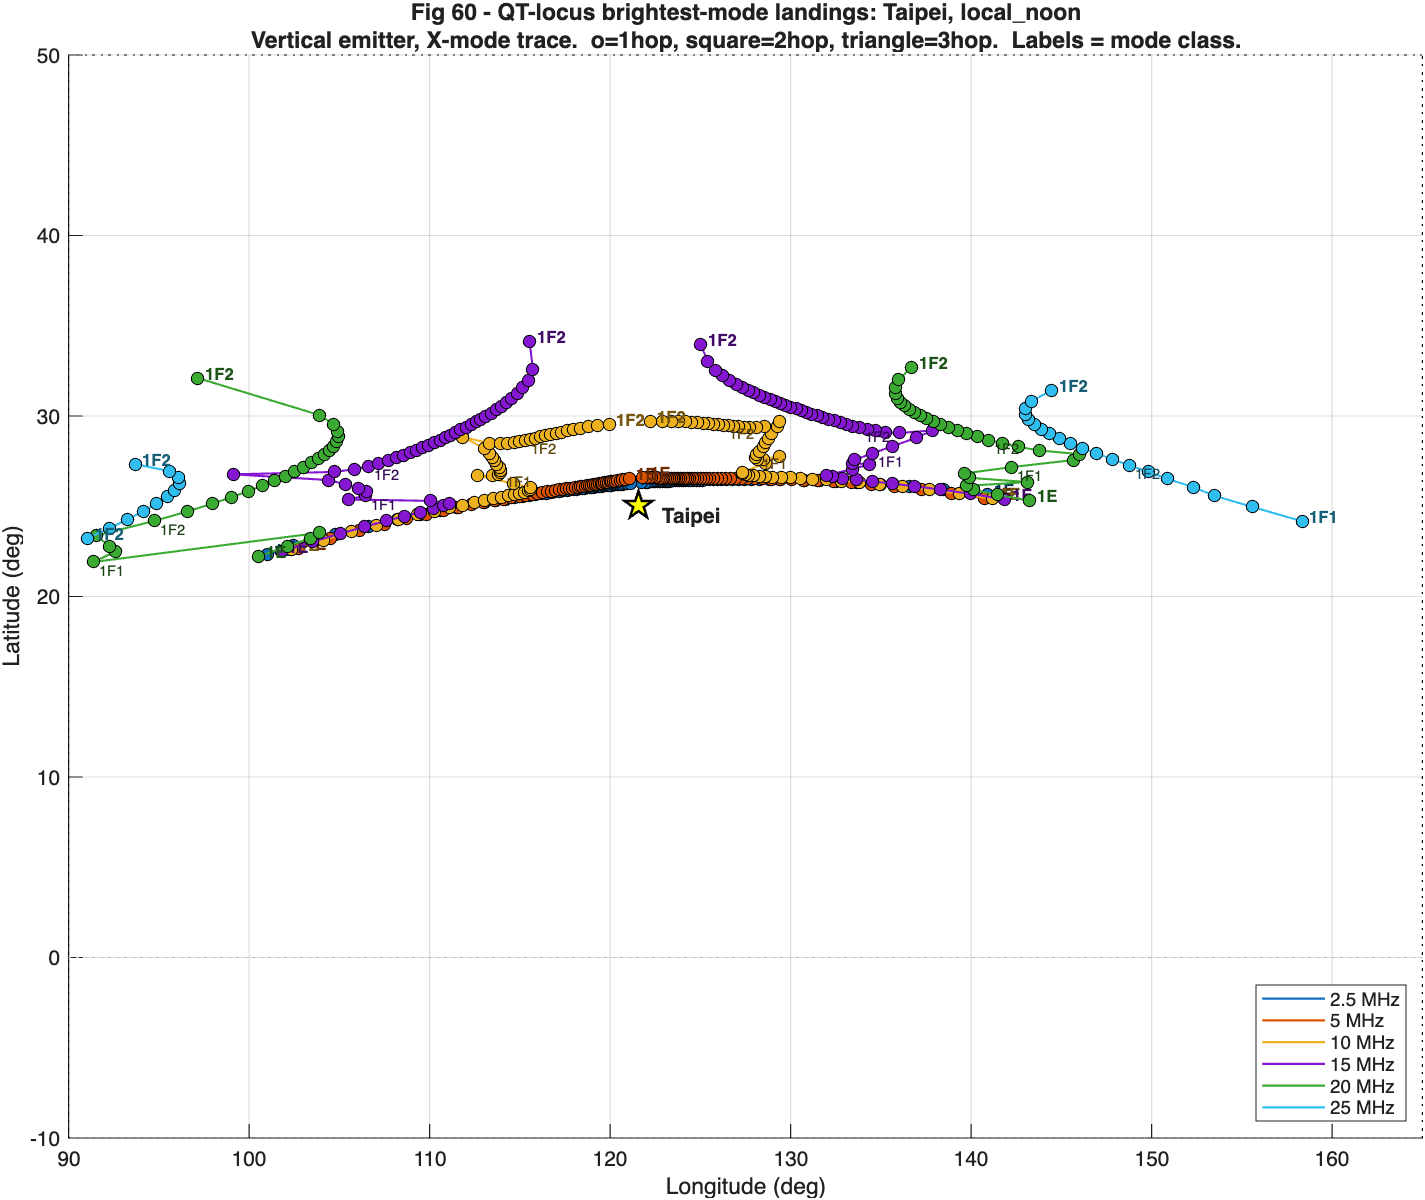
\includegraphics[width=\textwidth]{taipei_qt_map_noon.png}\\
\textbf{(a)} local noon
\end{minipage}\hfill
\begin{minipage}{0.49\textwidth}\centering
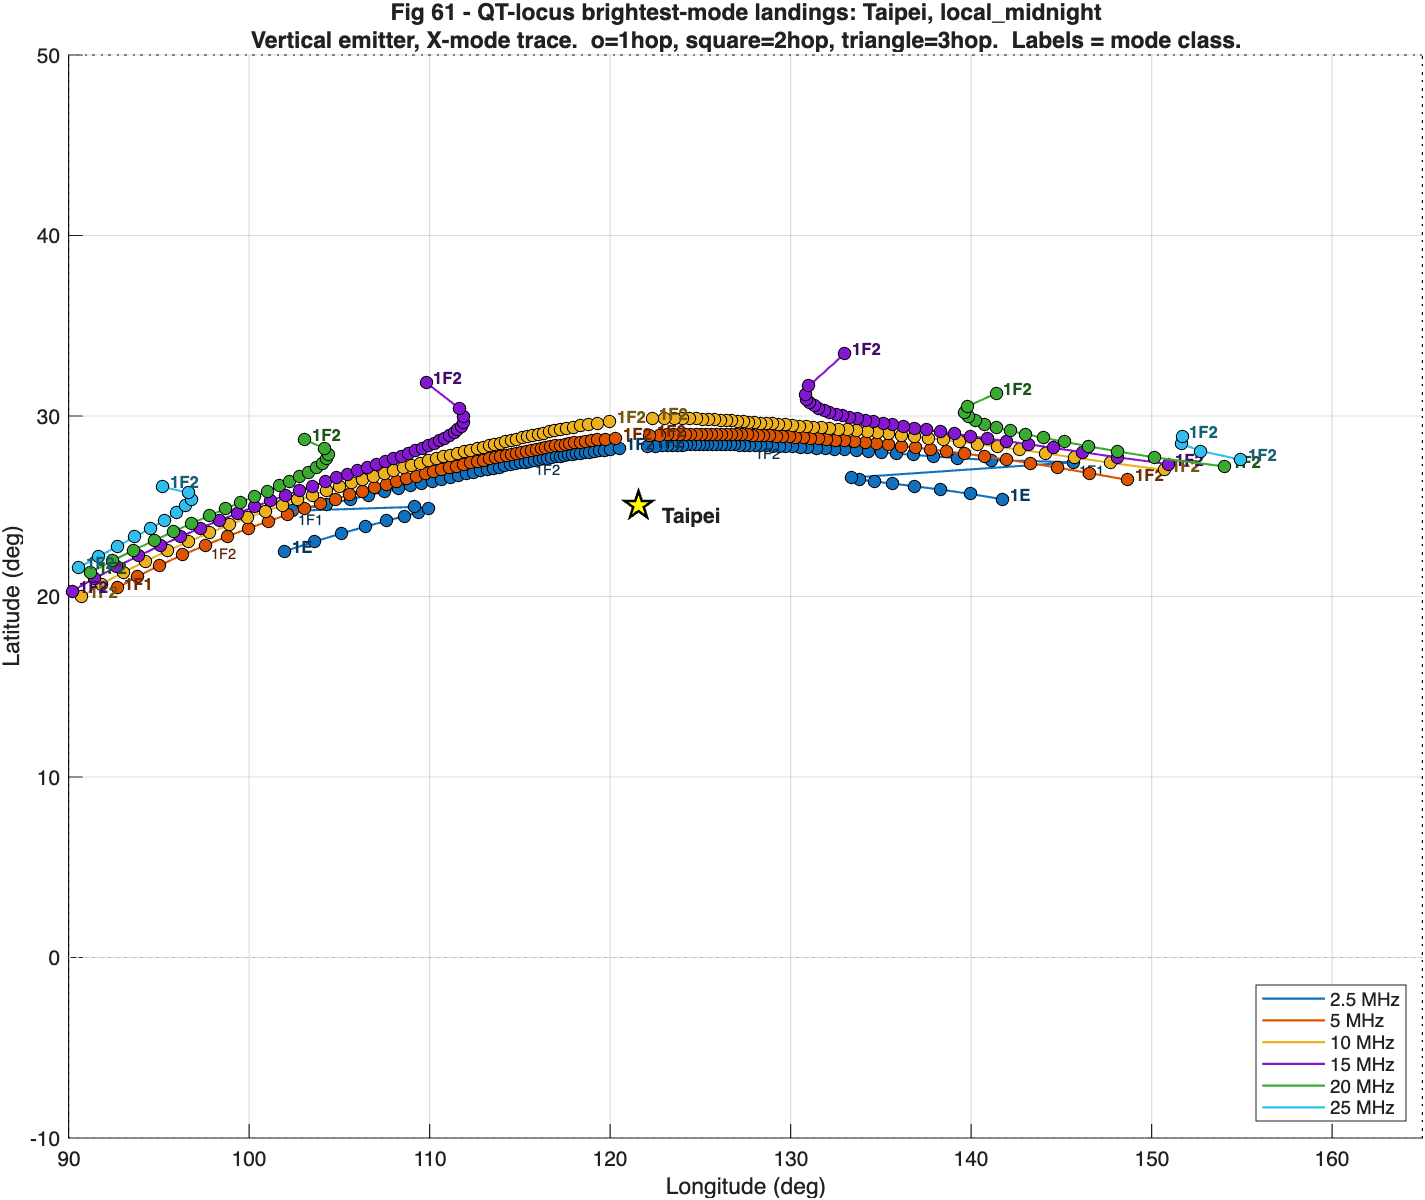
\includegraphics[width=\textwidth]{taipei_qt_map_midnight.png}\\
\textbf{(b)} local midnight
\end{minipage}
\caption{QT-locus brightest-mode landings from Taipei, on a flat
geographic projection.  Note the much wider arcs compared to FC --
the lower dip extends the locus to higher elevations and broader
azimuth coverage.  Equatorial-anomaly enhancement of the noon
ionosphere boosts daytime bands at lower frequencies; midnight is
quieter but with weaker F2-layer support.}
\label{fig:taipei_maps}
\end{figure}

\begin{figure}[H]
\centering
\begin{minipage}{0.49\textwidth}\centering
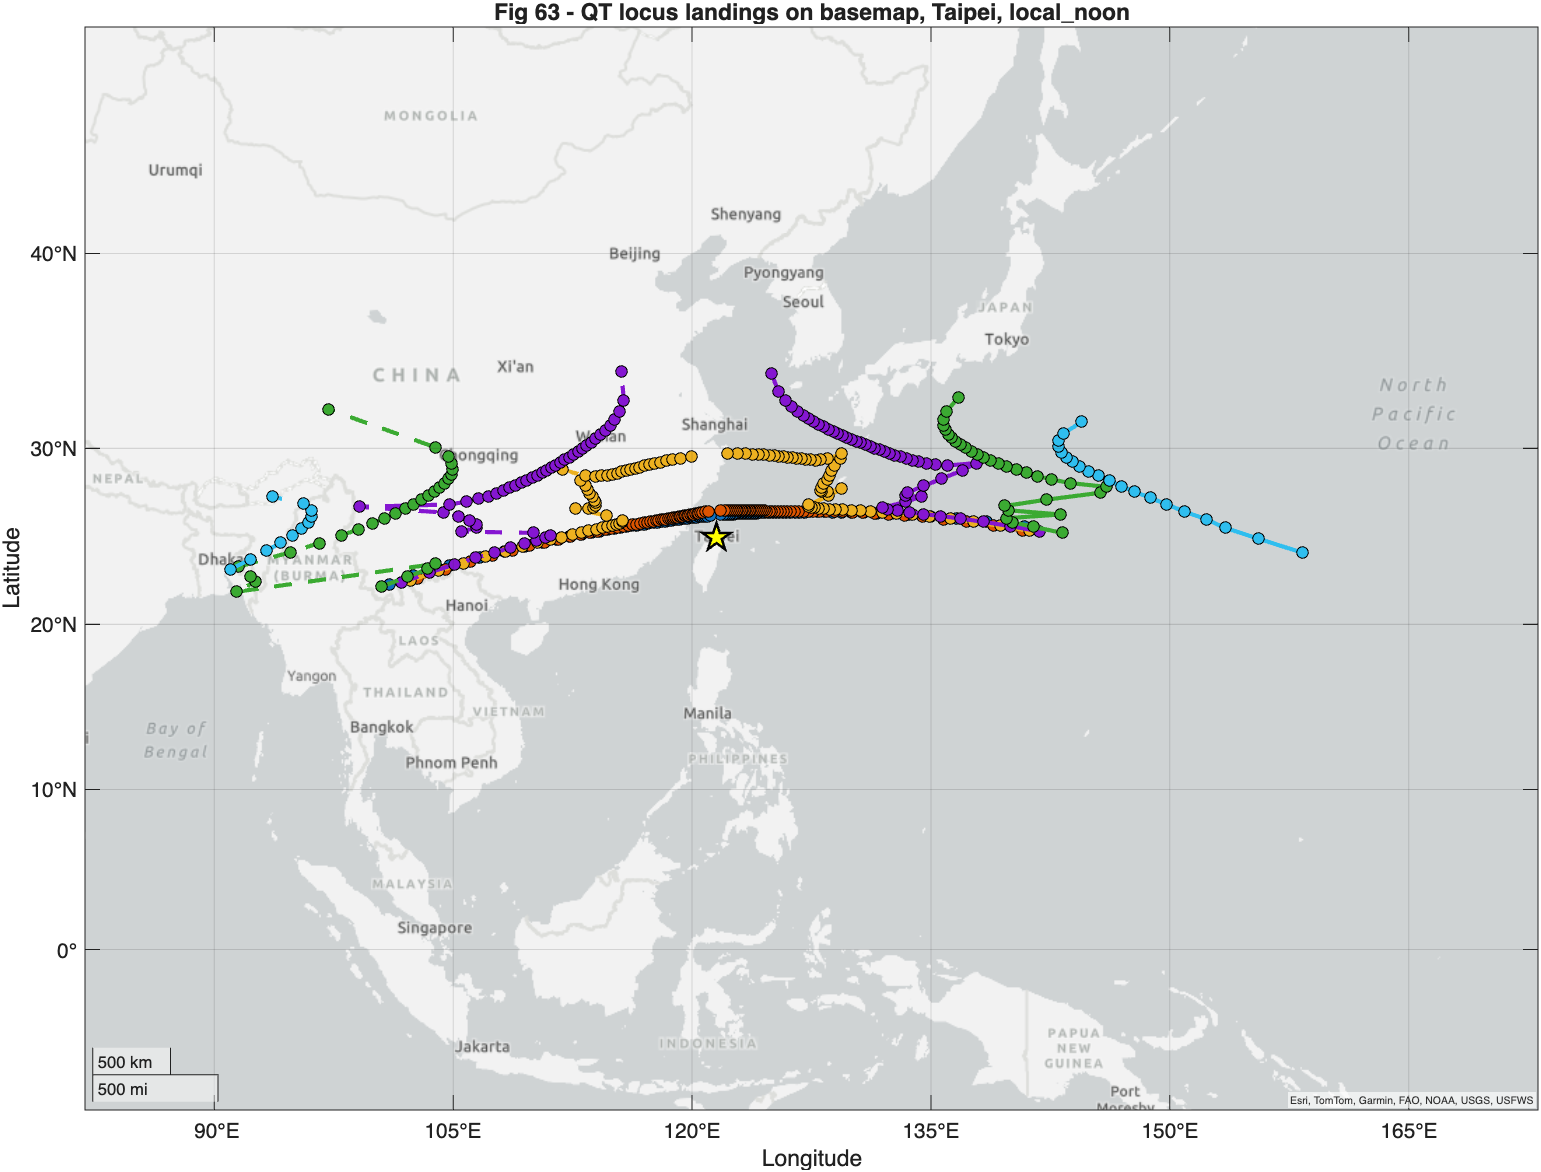
\includegraphics[width=\textwidth]{taipei_qt_basemap_noon.png}\\
\textbf{(a)} local noon
\end{minipage}\hfill
\begin{minipage}{0.49\textwidth}\centering
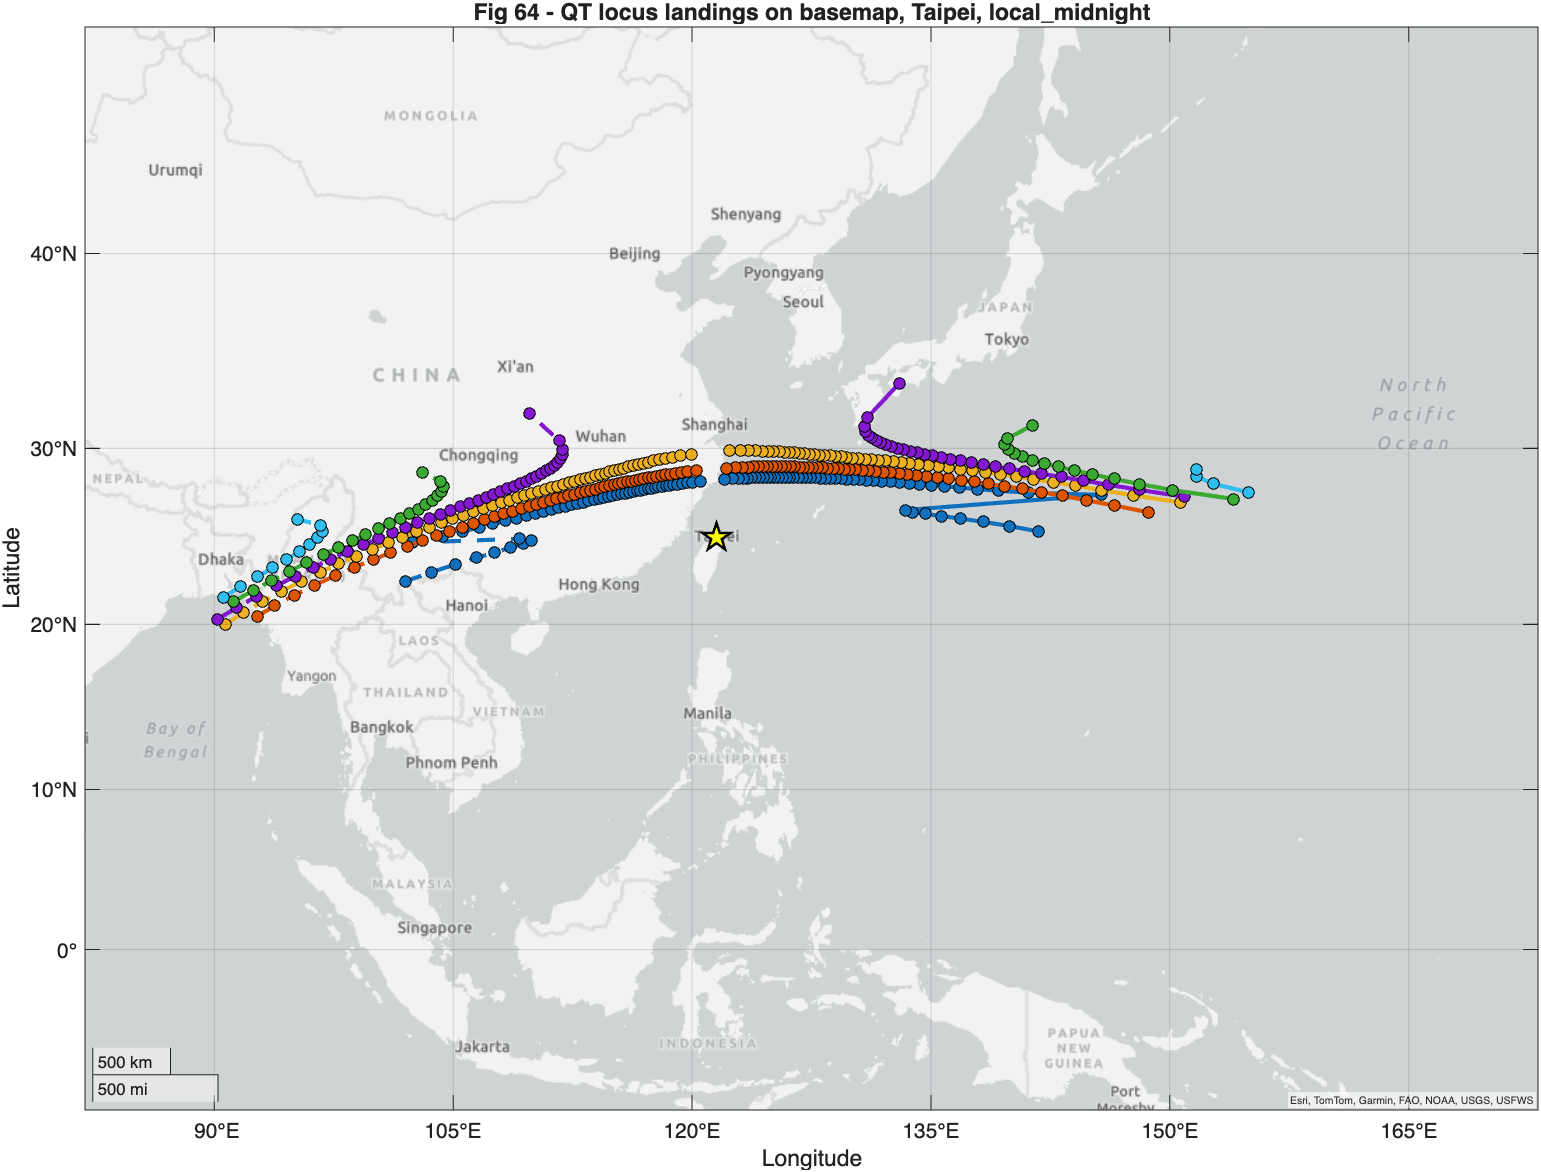
\includegraphics[width=\textwidth]{taipei_qt_basemap_midnight.png}\\
\textbf{(b)} local midnight
\end{minipage}
\caption{Same Taipei landings on a real basemap.  The locus reaches
into Japan, the Philippines, southern China, Vietnam, and well into
the western Pacific -- substantially wider geographic coverage than
the FC case, at the cost of weaker per-direction mode discrimination.}
\label{fig:taipei_basemaps}
\end{figure}

\begin{table}[H]
\centering
\caption{Brightest QT-locus ray per frequency, Taipei, local noon
(east branch).  The Taipei CSV pre-dates the addition of the
\texttt{mode\_ratio\_dB} column; the column reads as $0$ for that
reason.  The geometric ratio at Taipei's dip is $\approx +1.5\,$dB
plateau off-meridian, falling to $0$\,dB only as the launch
approaches the magnetic-meridian cutoff (where vertical-antenna
$\alpha\to 0$ but the modes are no longer purely linear because the
QL component grows).}
\begin{tabular}{rrrlrrrrr}
\toprule
$f$ & $\varepsilon$ & az & class & range & $b/a$ & $f_X/f_O$ & loss & lat,lon \\
MHz & deg & deg & & approx & & dB & dB & deg \\
\midrule
2.5 & 35.0 & 53.1 & 1E & 1-hop & 0.83 & +0.0 & -244.9 & 26.4, 123.6 \\
5.0 & 26.0 & 63.5 & 1E & 1-hop & 0.84 & +0.0 & -157.1 & 26.5, 125.0 \\
10.0 & 52.0 & 7.9 & 1F2 & 1-hop & 1.00 & +0.0 & -130.0 & 29.7, 122.2 \\
15.0 & 38.0 & 48.8 & 1F2 & 1-hop & 0.97 & +0.0 & -129.0 & 30.8, 129.2 \\
20.0 & 25.0 & 64.5 & 1F2 & 1-hop & 0.95 & +0.0 & -130.7 & 30.6, 136.3 \\
25.0 & 17.0 & 71.9 & 1F2 & 1-hop & 0.93 & +0.0 & -132.5 & 29.8, 143.2 \\
\bottomrule
\end{tabular}

\label{tab:taipei_noon}
\end{table}

\begin{table}[H]
\centering
\caption{Same as Table~\ref{tab:taipei_noon} but at local midnight.}
\begin{tabular}{rrrlrrrrr}
\toprule
$f$ & $\varepsilon$ & az & class & range & $b/a$ & $f_X/f_O$ & loss & lat,lon \\
MHz & deg & deg & & approx & & dB & dB & deg \\
\midrule
2.5 & 52.0 & 7.9 & 1F2 & 1-hop & 0.99 & +0.0 & -122.2 & 28.3, 122.1 \\
5.0 & 52.0 & 7.9 & 1F2 & 1-hop & 0.99 & +0.0 & -117.8 & 28.9, 122.2 \\
10.0 & 51.0 & 15.0 & 1F2 & 1-hop & 1.00 & +0.0 & -120.4 & 29.9, 123.0 \\
15.0 & 28.0 & 61.4 & 1F2 & 1-hop & 0.94 & +0.0 & -124.5 & 30.0, 132.9 \\
20.0 & 18.0 & 71.0 & 1F2 & 1-hop & 0.90 & +0.0 & -127.8 & 29.5, 140.8 \\
25.0 & 11.0 & 76.8 & 1F2 & 1-hop & 0.77 & +0.0 & -131.7 & 28.1, 152.7 \\
\bottomrule
\end{tabular}

\label{tab:taipei_midnight}
\end{table}


\section{Receiver-side polarization vs.\ frequency}

\begin{figure}[H]
\centering
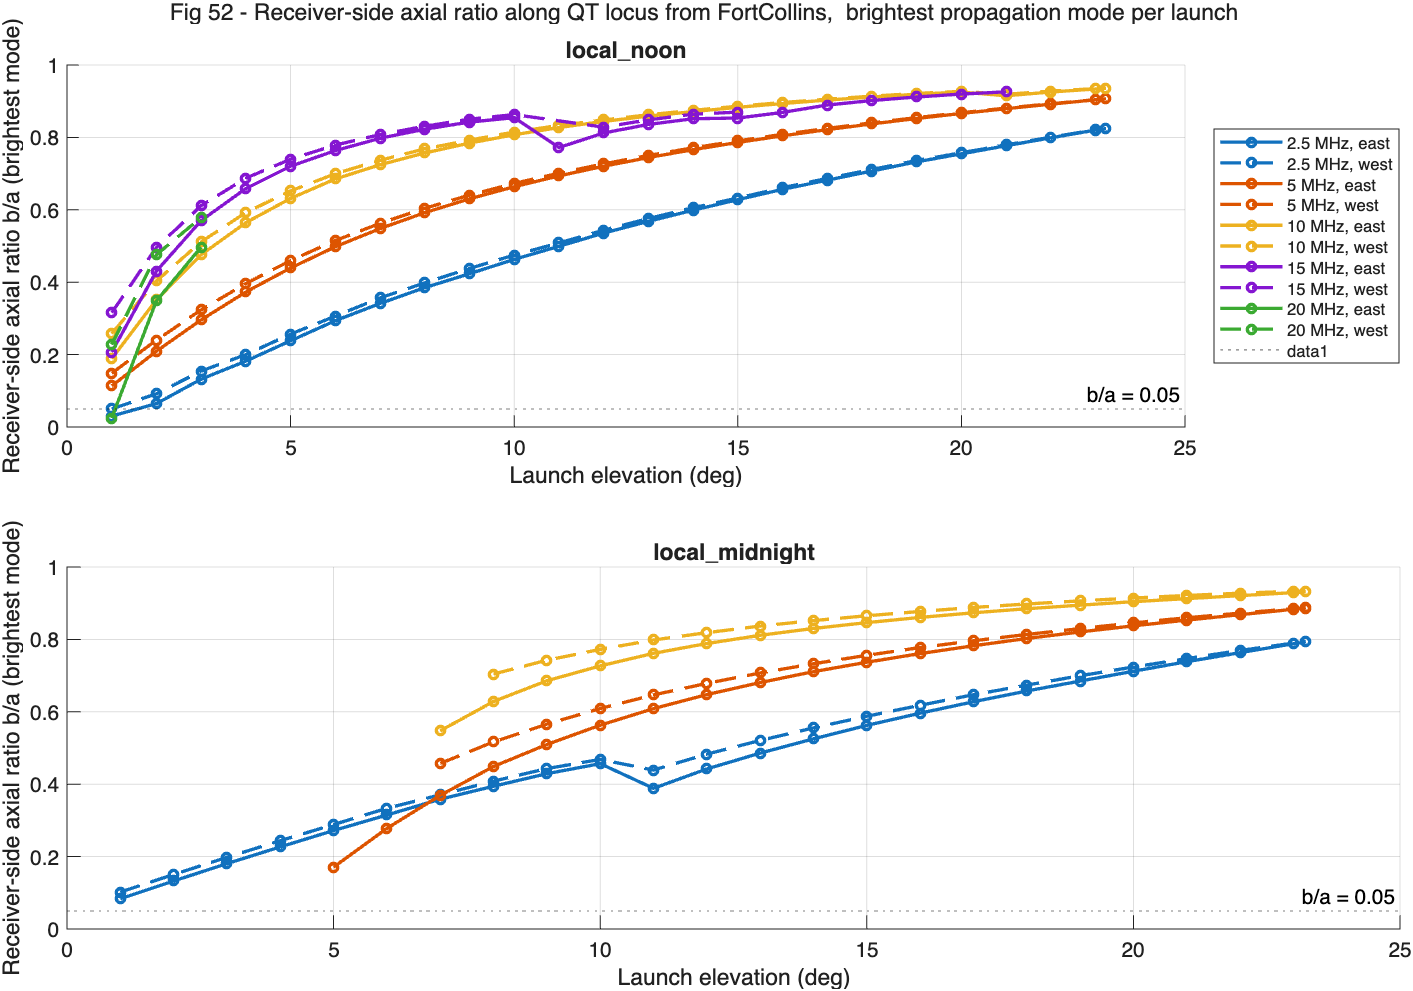
\includegraphics[width=0.95\textwidth]{qt_locus_polariz_state.png}
\caption{Receiver-side axial ratio $b/a$ along the QT locus from
Fort Collins, both branches, both times of day, all six frequencies.
The trend: at low frequency the modes are nearly linear at every
sample point along the path (deep-QT-effective regime), so $b/a$
stays near zero; at higher frequency $f_H/f$ shrinks and the modes
become more elliptical at the iono-exit point, so $b/a$ rises toward
unity.  The axial ratio also depends on the elevation along the locus
through the local $\theta(\hat{k}, \hat{B})$ at the iono-exit
sample.}
\label{fig:polariz}
\end{figure}


\section{Discussion: experimental implications}

\subsection*{Single-fixed-vertical-antenna comms architecture}

For an FCC Part-5 experimental transmission from FC, the magnetic-
meridian cutoff geometry (azimuth $\approx 8\textdegree$ true,
elevation $\approx 24\textdegree$) gives \emph{pure-O launch with no
special hardware}.  Skip distance is frequency-dependent: 5\,MHz
$\sim$800\,km, 10\,MHz $\sim$1100\,km, 15\,MHz $\sim$1250\,km,
20\,MHz $\sim$1400\,km.  All land roughly along the magnetic meridian
toward Saskatchewan / Manitoba; together they form a fan of
single-mode-pure landing sites that a frequency-agile transmitter can
hop between as the diurnal ionosphere evolves.

\subsection*{Off-meridian QT directions: shallower but useful}

If the receiver location is fixed and not on the magnetic meridian
(e.g., a KiwiSDR you happen to like), the rest of the QT locus still
provides $\approx +7\,$dB X-mode preference (or $-7\,$dB O-mode
preference for a horizontal antenna).  This is enough to do
\emph{differential} mode-coherence measurements but not enough to do
absolute single-mode propagation studies without additional rejection
at the receiver (e.g., orthogonal-magloop polarization decomposition;
see the receiver architecture in the project README).

\subsection*{Taipei vs.\ FC: complementary strengths}

The lower dip at Taipei ($\sim 36\textdegree$) makes mode
discrimination weaker per direction (only $\sim +1.5\,$dB plateau)
but extends the QT locus to much higher launch elevations and a
much wider azimuth coverage.  An equatorial-anomaly site is the
\emph{wrong} choice if you want maximum single-mode purity but the
\emph{right} choice if you want to survey many receive directions
along QT with one antenna.

\subsection*{What the geometry can't give you}

\begin{itemize}
\item The QL-circular geometry ($\hat{k}\!\parallel\!\hat{B}$) is
  achievable only by transmitting toward magnetic SOUTH at elevation
  equal to the dip (down toward the dip pole, looking up at
  elevation = dip).  At FC that's mag-S at $66\textdegree$
  elevation -- a real launch direction, but it gives 50/50 mode
  excitation for any linear antenna and so is useless for
  mode-discrimination purposes.  Useful only as a
  \emph{calibration} geometry where O and X are known to be
  excited equally.
\item Pure single-mode launch in arbitrary directions requires
  electronic polarization control at the transmitter (e.g.,
  crossed-dipole feeds with adjustable amplitude ratio).  Not
  required if the receiver does the mode separation in software --
  see the orthogonal-magloop architecture documented elsewhere in
  this repository.
\end{itemize}


\section*{Reproducibility}

Source MATLAB / Python scripts and CSV / KML data products live in
\texttt{\textasciitilde/Documents/MATLAB/pharlap/} (PHaRLAP work) and
\texttt{\textasciitilde/Desktop/projects/ionosphere/kiwiclient/}
(supporting tools).  Specifically:

\begin{itemize}
\item \texttt{pharlap\_qt\_locus.m} -- FC QT-locus enumeration with
  per-frequency map and KML export.
\item \texttt{pharlap\_qt\_locus\_taipei.m} -- Taipei equivalent.
\item \texttt{qt\_polar\_map.py} -- the Stokes-style polar map,
  pure-Python (no PHaRLAP dependency).
\item \texttt{build\_qt\_report\_tables.py} -- regenerate the LaTeX
  table fragments from the CSV outputs.
\end{itemize}

To regenerate this report:
\begin{verbatim}
# 1. Run the MATLAB scripts to (re)generate the CSVs and PNGs in
#    ~/Documents/MATLAB/pharlap/batch_out/
# 2. Then:
cd hf-polarimetry-release/reports/qt_locus
python3 ~/Documents/MATLAB/pharlap/build_qt_report_tables.py
pdflatex qt_locus_report.tex
pdflatex qt_locus_report.tex   # second pass for cross-refs
\end{verbatim}


\section*{References}

\begin{itemize}
\item Cervera, M.~A., \textit{PHaRLAP -- a HF radio propagation
  ray-tracing toolkit}, Defence Sci.\ \& Tech.\ Group, Australia.
\item Davies, K.\ (1990), \textit{Ionospheric Radio}, IEE
  Electromagnetic Waves Series 31.
\item Phillips \& Knight (1965), Proc.\ IEE \textbf{112}(1), 31--39.
\item Pederick, L.~H.\ \& Cervera, M.~A.\ (2014), Radio Sci.\
  \textbf{49}, 81--93.
\item Bilitza, D.\ (2018), \textit{The International Reference
  Ionosphere -- IRI 2020}, Space Sci.\ Rev.
\end{itemize}

\end{document}
